\documentclass[tikz,border=4pt]{standalone}

\usepackage[T1]{fontenc}
\usepackage{amsmath,amssymb}
\usepackage{helvet}
\renewcommand{\familydefault}{\sfdefault}

\usetikzlibrary{
  arrows.meta,
  backgrounds,
  calc,
  decorations.pathreplacing,
  positioning
}

% ---------------------------------------------------------------------------
% Neutral white canvas with navy structure and ruby spin arrows.
% Change these definitions to recolor the complete figure.
% ---------------------------------------------------------------------------
\definecolor{canvas}{HTML}{FFFFFF}
\definecolor{ink}{HTML}{252C35}
\definecolor{navy}{HTML}{30465B}
\definecolor{steel}{HTML}{607F98}
\definecolor{sky}{HTML}{A8C1D1}
\definecolor{mist}{HTML}{E8EEF2}
\definecolor{warmgray}{HTML}{D8D2C8}
\definecolor{weakgray}{HTML}{AAB2B8}
\definecolor{ruby}{HTML}{A30F18}
\definecolor{rose}{HTML}{F3E2E1}
\definecolor{gold}{HTML}{B2863B}
\definecolor{palegold}{HTML}{F3EAD7}

\tikzset{
  >={Latex[length=2.2mm,width=1.5mm]},
  panel/.style={
    draw=navy,
    line width=.75pt,
    rounded corners=4mm,
    fill=white
  },
  inset/.style={
    draw=steel,
    line width=.55pt,
    rounded corners=2mm,
    fill=canvas
  },
  section title/.style={font=\bfseries\large, text=navy},
  panel title/.style={font=\bfseries\fontsize{16}{18}\selectfont},
  small title/.style={font=\bfseries\small, text=navy},
  body/.style={font=\small, text=ink},
  tiny body/.style={font=\footnotesize, text=ink},
  flow/.style={-Latex, draw=ink, line width=1.1pt},
  blue flow/.style={-Latex, draw=steel, line width=1.15pt},
  weak edge/.style={draw=weakgray, line width=.55pt},
  edge/.style={draw=ink, line width=.7pt},
  strong edge/.style={draw=ink, line width=1.45pt},
  directed edge/.style={
    -{Stealth[length=2.05mm,width=1.50mm]},
    draw=ink,
    line width=.7pt,
    shorten <=3.1mm,
    shorten >=4.6mm
  },
  weak directed/.style={
    -{Stealth[length=1.85mm,width=1.30mm]},
    draw=weakgray,
    line width=.5pt,
    shorten <=3.1mm,
    shorten >=4.6mm
  },
  strong directed/.style={
    -{Stealth[length=2.35mm,width=1.70mm]},
    draw=ink,
    line width=1.45pt,
    shorten <=3.1mm,
    shorten >=4.8mm
  },
  spinnode/.style={
    circle,
    draw=ink,
    fill=white,
    line width=.6pt,
    minimum size=7.5mm,
    inner sep=0pt
  },
  spin arrow/.style={
    -{Latex[length=2.85mm,width=1.95mm]},
    draw=ruby,
    line width=1.65pt,
    line cap=round
  },
  cycle block/.style={
    draw=navy,
    fill=mist,
    rounded corners=2mm,
    line width=.75pt,
    minimum height=1.55cm
  },
  block/.style={
    draw=navy,
    fill=white,
    rounded corners=1mm,
    line width=.7pt,
    minimum width=1.25cm,
    minimum height=.55cm
  }
}

% A vector-spin site in the visual language of vector_spins.png.
% Usage: \Spin{name}{(x,y)}{angle in degrees}
\newcommand{\Spin}[3]{%
  \node[spinnode] (#1) at #2 {};
  \draw[spin arrow] (#1.center) -- ++(#3:0.62);
}

% Numbered panel heading.
\newcommand{\PanelHeading}[4]{%
  \node[circle,fill=#4,text=white,font=\bfseries\Large,
        minimum size=8mm,inner sep=0pt] at (#1,#2) {#3};
}

\begin{document}
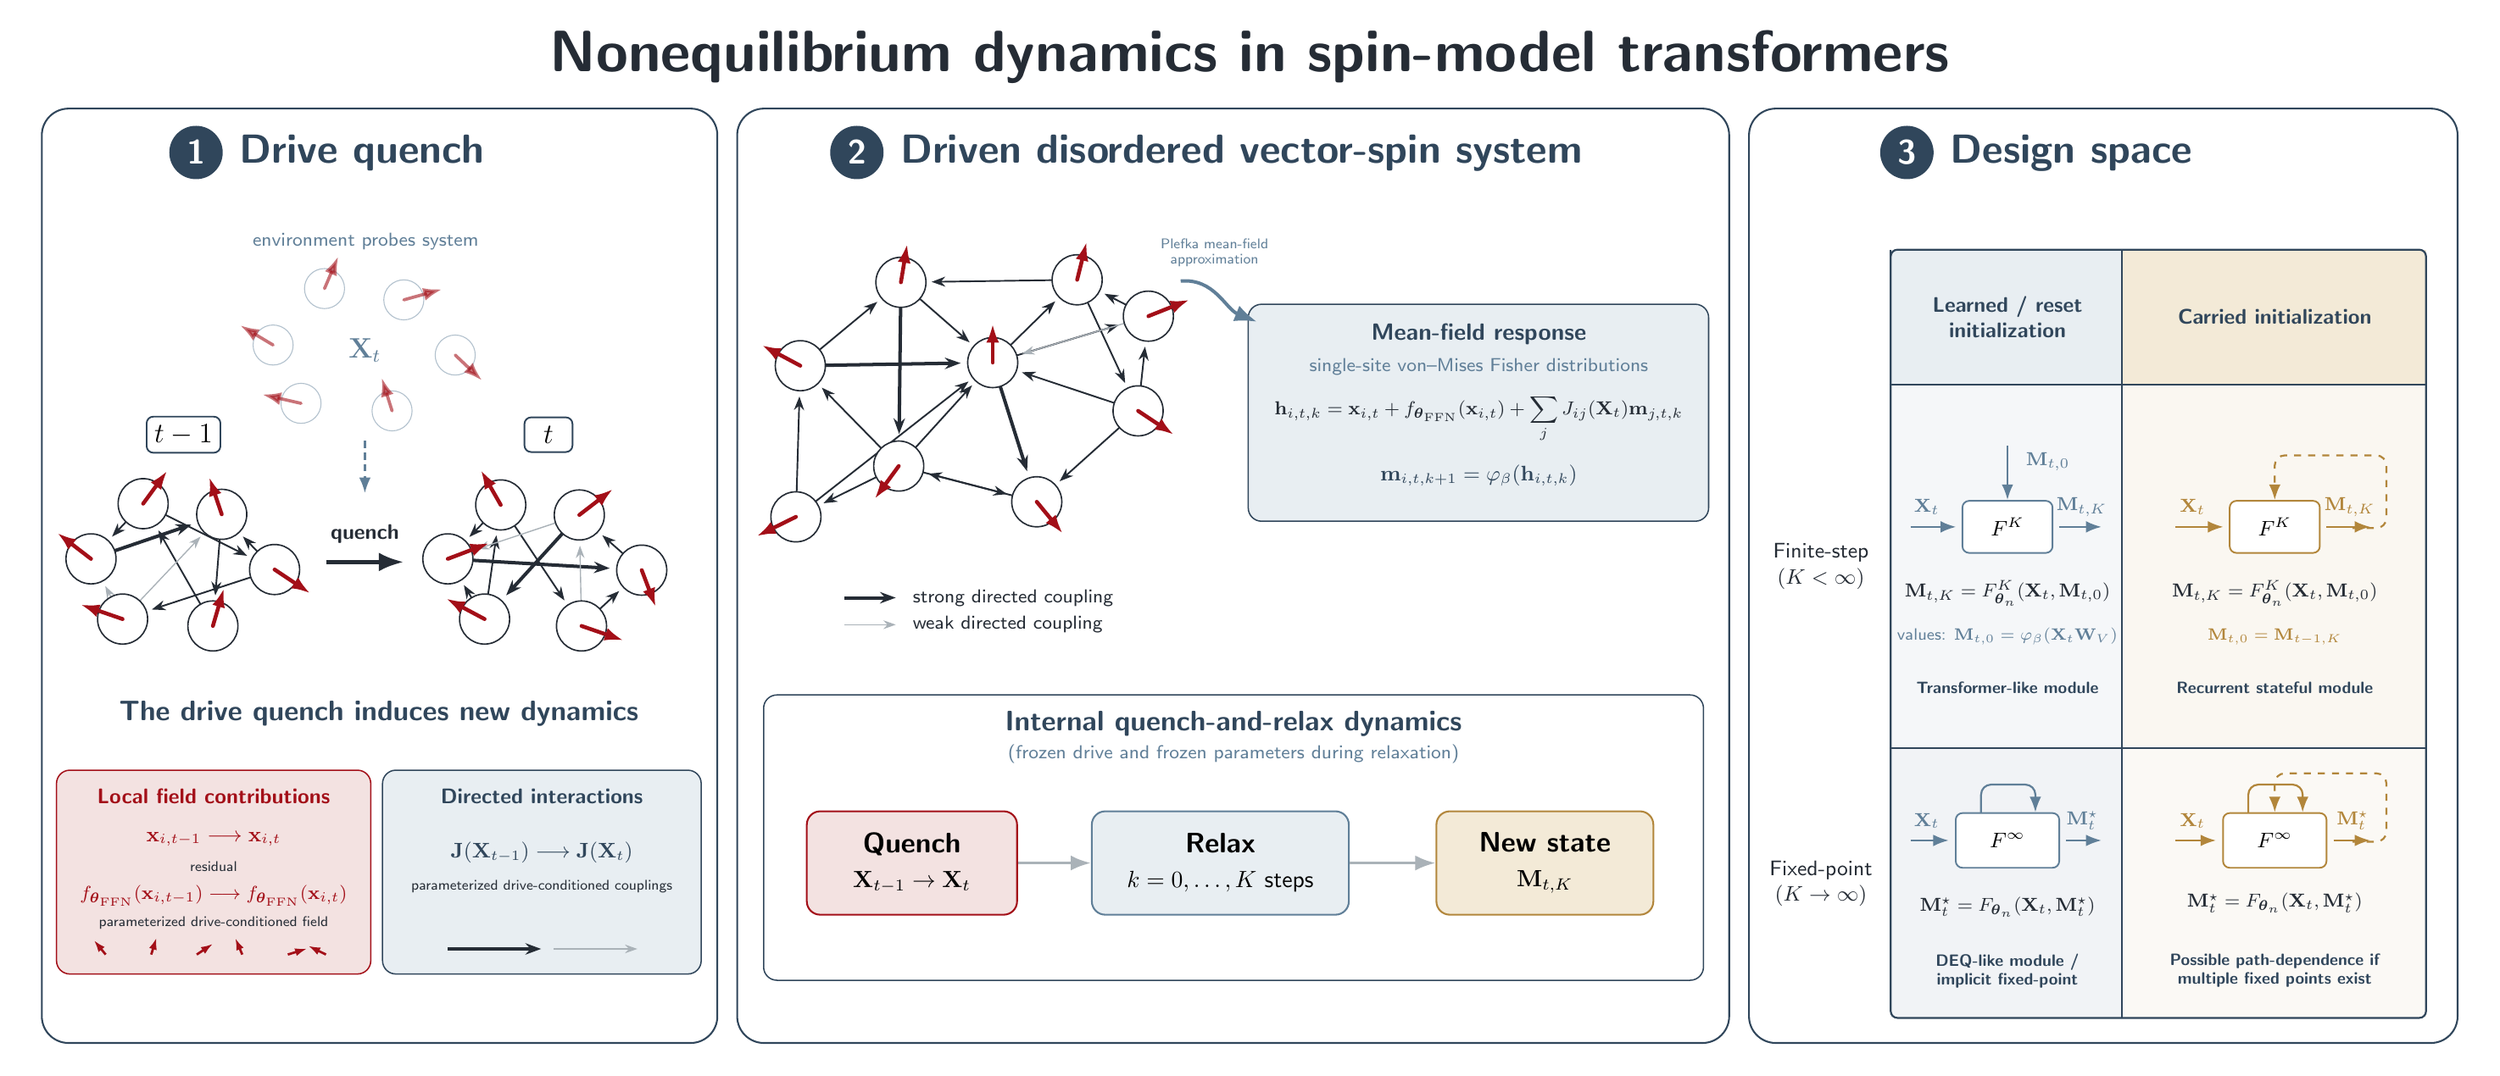
\begin{tikzpicture}[x=1.10cm,y=.94cm]

  % Canvas -----------------------------------------------------------------
  \fill[canvas] (0,1.80) rectangle (33.4,18.2);
  \node[font=\bfseries\fontsize{23}{26}\selectfont,text=ink]
    at (16.7,17.67) {Nonequilibrium dynamics in spin-model transformers};

  % Main panels -------------------------------------------------------------
  \draw[panel] (.25,1.95) rectangle (9.45,16.85);
  \draw[panel] (9.72,1.95) rectangle (23.23,16.85);
  \draw[panel] (23.50,1.95) rectangle (33.15,16.85);

  % ------------------------------------------------------------------------
  % 1. DRIVE QUENCH
  % ------------------------------------------------------------------------
  \PanelHeading{2.35}{16.15}{1}{navy}
  \node[panel title,text=navy,anchor=west]
    at (2.83,16.14) {Drive quench};

  % One faded drive-only system represents the outside environment probing
  % the interacting system at the quench.  It carries no interaction edges.
  \node[tiny body,text=steel] at (4.66,14.73)
    {environment probes system};
  \coordinate (ega) at (3.40,13.08); \coordinate (egb) at (4.10,13.98);
  \coordinate (egc) at (5.18,13.80); \coordinate (egd) at (5.88,12.92);
  \coordinate (ege) at (5.02,12.03); \coordinate (egf) at (3.78,12.15);
  \foreach \p in {ega,egb,egc,egd,ege,egf}
    \node[circle,draw=steel,fill=white,opacity=.48,
          minimum size=6.0mm,inner sep=0pt] at (\p) {};
  \foreach \p/\ang in {ega/145,egb/70,egc/18,egd/-48,ege/105,egf/165}
    \draw[spin arrow,opacity=.58,line width=1.35pt] (\p) -- ++(\ang:.55);
  \node[font=\large,text=steel] at (4.65,13.00) {$\mathbf{X}_t$};
  \draw[-Latex,draw=steel,densely dashed,line width=.8pt]
    (4.65,11.55) -- (4.65,10.72);

  % Solid interacting systems beneath the drive-only copies.
  \coordinate (qa) at (.92,9.67); \coordinate (qb) at (1.63,10.55);
  \coordinate (qc) at (2.70,10.38); \coordinate (qd) at (3.42,9.50);
  \coordinate (qe) at (2.58,8.60); \coordinate (qf) at (1.35,8.71);
  \coordinate (ra) at (5.78,9.67); \coordinate (rb) at (6.50,10.53);
  \coordinate (rc) at (7.57,10.37); \coordinate (rd) at (8.42,9.49);
  \coordinate (re) at (7.60,8.60); \coordinate (rf) at (6.28,8.71);

  \draw[strong directed] (qa)--(qc);
  \foreach \a/\b in {qb/qa,qb/qd,qc/qe,qd/qc,qd/qf,qe/qb}
    \draw[directed edge] (\a)--(\b);
  \foreach \a/\b in {qf/qa,qf/qc}
    \draw[weak directed] (\a)--(\b);
  \foreach \a/\b in {ra/rd,rc/rf}
    \draw[strong directed] (\a)--(\b);
  \foreach \a/\b in {rb/ra,rb/re,rd/rc,re/rd,rf/rb,rf/ra}
    \draw[directed edge] (\a)--(\b);
  \foreach \a/\b in {rc/ra,re/rc}
    \draw[weak directed] (\a)--(\b);

  \Spin{qan}{(qa)}{138} \Spin{qbn}{(qb)}{58} \Spin{qcn}{(qc)}{106}
  \Spin{qdn}{(qd)}{-38} \Spin{qen}{(qe)}{76} \Spin{qfn}{(qf)}{158}
  \Spin{ran}{(ra)}{24} \Spin{rbn}{(rb)}{116} \Spin{rcn}{(rc)}{42}
  \Spin{rdn}{(rd)}{-72} \Spin{ren}{(re)}{-22} \Spin{rfn}{(rf)}{148}

  \node[block,draw=navy,fill=white,minimum width=.92cm,
        minimum height=.52cm,font=\large] at (2.18,11.65) {$t-1$};
  \node[block,draw=navy,fill=white,minimum width=.72cm,
        minimum height=.52cm,font=\large] at (7.15,11.65) {$t$};

  \draw[flow,line width=1.7pt] (4.12,9.62) -- (5.18,9.62);
  \node[body,font=\bfseries\small,above=1.5mm] at (4.65,9.62) {quench};

  \node[section title] at (4.84,7.20)
    {The drive quench induces new dynamics};

  \draw[inset,draw=ruby,fill=rose] (.45,3.05) rectangle (4.73,6.30);
  \node[small title,text=ruby] at (2.59,5.88) {Local field contributions};
  \node[body,text=ruby] at (2.59,5.20)
    {$\mathbf{x}_{i,t-1}\longrightarrow\mathbf{x}_{i,t}$};
  \node[tiny body,font=\fontsize{6.5}{7.3}\selectfont] at (2.59,4.77)
    {residual};
  \node[tiny body,text=ruby] at (2.59,4.30)
    {$f_{\boldsymbol{\theta}_{\mathrm{FFN}}}(\mathbf{x}_{i,t-1})
      \longrightarrow
      f_{\boldsymbol{\theta}_{\mathrm{FFN}}}(\mathbf{x}_{i,t})$};
  \node[tiny body,font=\fontsize{6.5}{7.3}\selectfont] at (2.59,3.87)
    {parameterized drive-conditioned field};
  \foreach \x/\ang in {1.12/125,1.74/75,2.36/38,2.98/110,3.60/20,4.12/150}
    \draw[-{Latex[length=1.8mm,width=1.2mm]},draw=ruby,line width=1.0pt]
      (\x,3.36) -- ++(\ang:.28);

  \draw[inset,draw=navy,fill=mist] (4.89,3.05) rectangle (9.23,6.30);
  \node[small title] at (7.06,5.88) {Directed interactions};
  \node[body,align=center,text=navy] at (7.06,4.98)
    {$\mathbf{J}(\mathbf{X}_{t-1})
      \longrightarrow\mathbf{J}(\mathbf{X}_t)$};
  \node[tiny body,font=\fontsize{6.5}{7.3}\selectfont] at (7.06,4.45)
    {parameterized drive-conditioned couplings};
  \draw[strong directed,shorten <=0mm,shorten >=0mm]
    (5.78,3.45) -- (7.05,3.45);
  \draw[weak directed,shorten <=0mm,shorten >=0mm]
    (7.22,3.45) -- (8.36,3.45);

  % ------------------------------------------------------------------------
  % 2. DRIVEN DISORDERED VECTOR-SPIN SYSTEM
  % ------------------------------------------------------------------------
  \PanelHeading{11.35}{16.15}{2}{navy}
  \node[panel title,text=navy,anchor=west]
    at (11.83,16.14) {Driven disordered vector-spin system};

  % Coupling graph: edges first, then vector-spin sites.
  \coordinate (s1) at (10.58,12.75);
  \coordinate (s2) at (11.95,14.08);
  \coordinate (s3) at (14.35,14.12);
  \coordinate (s4) at (13.20,12.80);
  \coordinate (s5) at (15.18,12.03);
  \coordinate (s6) at (11.92,11.15);
  \coordinate (s7) at (13.80,10.58);
  \coordinate (s8) at (10.52,10.34);
  \coordinate (s9) at (15.32,13.54);

  \foreach \a/\b in {s1/s4,s2/s6,s4/s7}
    \draw[strong directed] (\a)--(\b);
  \foreach \a/\b in {
      s1/s2,s3/s2,s3/s5,s5/s7,s6/s7,s6/s1,
      s2/s4,s4/s3,s5/s4,s6/s4,s7/s6,
      s8/s1,s6/s8,s8/s4,s9/s3,s5/s9,s4/s9}
    \draw[directed edge] (\a)--(\b);
  \draw[weak directed] (s9)--(s4);

  \Spin{s1n}{(s1)}{148}
  \Spin{s2n}{(s2)}{82}
  \Spin{s3n}{(s3)}{78}
  \Spin{s4n}{(s4)}{90}
  \Spin{s5n}{(s5)}{-38}
  \Spin{s6n}{(s6)}{-122}
  \Spin{s7n}{(s7)}{-55}
  \Spin{s8n}{(s8)}{-150}
  \Spin{s9n}{(s9)}{25}

  \draw[strong directed,shorten <=0mm,shorten >=0mm]
    (11.18,9.05) -- (11.88,9.05);
  \node[tiny body,anchor=west] at (12.00,9.05) {strong directed coupling};
  \draw[weak directed,shorten <=0mm,shorten >=0mm]
    (11.18,8.62) -- (11.88,8.62);
  \node[tiny body,anchor=west] at (12.00,8.62) {weak directed coupling};

  % Local effective field followed by the one-site mean-field response.
  \draw[inset,draw=navy,fill=mist] (16.68,10.27) rectangle (22.95,13.73);
  \node[font=\bfseries\normalsize,text=navy] at (19.82,13.25)
    {Mean-field response};
  \node[tiny body,text=steel] at (19.82,12.73)
    {single-site von--Mises Fisher distributions};
  \node[tiny body,align=center] at (19.82,11.90)
    {$\mathbf{h}_{i,t,k}=\mathbf{x}_{i,t}
       +f_{\boldsymbol{\theta}_{\mathrm{FFN}}}(\mathbf{x}_{i,t})
       +\displaystyle\sum_j J_{ij}(\mathbf{X}_t)\mathbf{m}_{j,t,k}$};
  \node[body,align=center,text=navy] at (19.82,11.00)
    {$\mathbf{m}_{i,t,k+1}
      =\varphi_{\beta}(\mathbf{h}_{i,t,k})$};
  \draw[flow,draw=steel,line width=1.45pt]
    (15.76,14.10) to[out=5,in=158] (16.80,13.45);
  \node[font=\fontsize{6.2}{6.8}\selectfont,text=steel,align=center,
        fill=white,inner sep=.7pt] at (16.22,14.55)
    {Plefka mean-field\\approximation};

  % Compact frozen-drive relaxation protocol.
  \draw[inset,draw=navy,fill=canvas] (10.08,2.95) rectangle (22.88,7.50);
  \node[section title] at (16.48,7.04)
    {Internal quench-and-relax dynamics};
  \node[tiny body,text=steel] at (16.48,6.56)
    {(frozen drive and frozen parameters during relaxation)};

  \node[cycle block,draw=ruby,fill=rose,minimum width=3.15cm,align=center]
    (quench) at (12.10,4.82)
    {{\bfseries\large Quench}\\[1mm]
     $\mathbf{X}_{t-1}\rightarrow\mathbf{X}_t$};
  \node[cycle block,draw=steel,fill=mist,minimum width=3.85cm,align=center]
    (relax) at (16.30,4.82)
    {{\bfseries\large Relax}\\[1mm]
     $k=0,\ldots,K$ steps};
  \node[cycle block,draw=gold,fill=palegold,minimum width=3.25cm,align=center]
    (newstate) at (20.72,4.82)
    {{\bfseries\large New state}\\[1mm]
     $\mathbf{M}_{t,K}$};

  \draw[flow,draw=weakgray,line width=1.25pt]
    (quench.east) -- (relax.west);
  \draw[flow,draw=weakgray,line width=1.25pt]
    (relax.east) -- (newstate.west);

  % ------------------------------------------------------------------------
  % 3. DESIGN SPACE
  % ------------------------------------------------------------------------
  \PanelHeading{25.65}{16.15}{3}{navy}
  \node[panel title,text=navy,anchor=west]
    at (26.13,16.14) {Design space};

  % Table geometry: blue-gray reset column, warm carried-state column.
  \fill[mist]       (25.43,12.45) rectangle (28.58,14.60);
  \fill[palegold]   (28.58,12.45) rectangle (32.72,14.60);
  \fill[steel!6]    (25.43,6.65) rectangle (28.58,12.45);
  \fill[gold!7]     (28.58,6.65) rectangle (32.72,12.45);
  \fill[steel!9]    (25.43,2.35) rectangle (28.58,6.65);
  \fill[gold!5]     (28.58,2.35) rectangle (32.72,6.65);
  \draw[draw=navy,line width=.8pt,rounded corners=1mm]
    (25.43,2.35) rectangle (32.72,14.60);
  \draw[navy,line width=.6pt] (28.58,2.35) -- (28.58,14.60);
  \draw[navy,line width=.6pt] (25.43,12.45) -- (32.72,12.45);
  \draw[navy,line width=.6pt] (25.43,6.65) -- (32.72,6.65);
  \draw[navy,line width=.6pt] (25.43,14.60) -- (25.43,12.45);

  \node[small title,text=navy,align=center] at (27.02,13.53)
    {Learned / reset\\initialization};
  \node[small title,text=navy,align=center] at (30.66,13.53)
    {Carried initialization};
  \node[body,align=center] at (24.48,9.55) {Finite-step\\$(K<\infty)$};
  \node[body,align=center] at (24.48,4.49) {Fixed-point\\$(K\to\infty)$};

  % Top-left: one finite-horizon module with reset/learned initialization.
  \node[block,draw=steel,fill=white,minimum width=1.35cm,
        minimum height=.78cm,font=\small] (fkL) at (27.02,10.18) {$F^K$};
  \draw[-Latex,draw=steel,line width=.8pt] (25.70,10.18) -- (26.32,10.18);
  \node[tiny body,text=steel] at (25.92,10.50) {$\mathbf{X}_t$};
  \draw[-Latex,draw=steel,line width=.8pt] (27.02,11.48) -- (27.02,10.61);
  \node[tiny body,text=steel,anchor=west] at (27.16,11.22)
    {$\mathbf{M}_{t,0}$};
  \draw[-Latex,draw=steel,line width=.8pt] (27.72,10.18) -- (28.30,10.18);
  \node[tiny body,text=steel] at (28.03,10.50) {$\mathbf{M}_{t,K}$};
  \node[tiny body,align=center,text=ink] at (27.02,9.12)
    {$\mathbf{M}_{t,K}=F^K_{\boldsymbol{\theta}_n}
      (\mathbf{X}_t,\mathbf{M}_{t,0})$};
  \node[tiny body,font=\scriptsize,text=steel,align=center] at (27.02,8.43)
    {values: $\mathbf{M}_{t,0}
       =\varphi_{\beta}(\mathbf{X}_t\mathbf{W}_{V})$};
  \node[small title,text=navy,align=center,font=\bfseries\scriptsize]
    at (27.02,7.62)
    {Transformer-like module};

  % Top-right: the same single module with carried-state feedback.
  \node[block,draw=gold,fill=white,minimum width=1.35cm,
        minimum height=.78cm,font=\small] (fkR) at (30.66,10.18) {$F^K$};
  \draw[-Latex,draw=gold,line width=.8pt] (29.30,10.18) -- (29.96,10.18);
  \node[tiny body,text=gold] at (29.54,10.50) {$\mathbf{X}_t$};
  \draw[-Latex,draw=gold,line width=.8pt] (31.36,10.18) -- (31.96,10.18);
  \node[tiny body,text=gold] at (31.68,10.50) {$\mathbf{M}_{t,K}$};
  \draw[-Latex,draw=gold,dashed,rounded corners=1.5mm,line width=.8pt]
    (31.72,10.16) -- (32.18,10.16) -- (32.18,11.32)
    -- (30.66,11.32) -- (30.66,10.61);
  \node[tiny body,align=center,text=ink] at (30.66,9.12)
    {$\mathbf{M}_{t,K}=F^K_{\boldsymbol{\theta}_n}
      (\mathbf{X}_t,\mathbf{M}_{t,0})$};
  \node[tiny body,font=\scriptsize,text=gold,align=center] at (30.66,8.43)
    {$\mathbf{M}_{t,0}=\mathbf{M}_{t-1,K}$};
  \node[small title,text=navy,align=center,font=\bfseries\scriptsize]
    at (30.66,7.62) {Recurrent stateful module};

  % Bottom-left: one implicit module solved to its fixed point.
  \node[block,draw=steel,fill=white,minimum width=1.55cm,
        minimum height=.82cm,font=\small] (finfL) at (27.02,5.18) {$F^{\infty}$};
  \draw[-Latex,draw=steel,line width=.8pt] (25.70,5.18) -- (26.22,5.18);
  \node[tiny body,text=steel] at (25.92,5.49) {$\mathbf{X}_t$};
  \draw[-Latex,draw=steel,line width=.8pt] (27.82,5.18) -- (28.30,5.18);
  \node[tiny body,text=steel] at (28.04,5.49) {$\mathbf{M}^{\star}_t$};
  \draw[-Latex,draw=steel,rounded corners=1.5mm,line width=.8pt]
    (26.66,5.62) -- (26.66,6.07) -- (27.40,6.07) -- (27.40,5.63);
  \node[tiny body,align=center] at (27.02,4.12)
    {$\mathbf{M}^{\star}_t=
      F_{\boldsymbol{\theta}_n}(\mathbf{X}_t,\mathbf{M}^{\star}_t)$};
  \node[small title,text=navy,align=center,font=\bfseries\scriptsize]
    at (27.02,3.10)
    {DEQ-like module /\\implicit fixed-point};

  % Bottom-right: the same fixed-point module with a carried warm start.
  \node[block,draw=gold,fill=white,minimum width=1.55cm,
        minimum height=.82cm,font=\small] (finfR) at (30.66,5.18) {$F^{\infty}$};
  \draw[-Latex,draw=gold,line width=.8pt] (29.30,5.18) -- (29.86,5.18);
  \node[tiny body,text=gold] at (29.54,5.49) {$\mathbf{X}_t$};
  \draw[-Latex,draw=gold,line width=.8pt] (31.46,5.18) -- (31.96,5.18);
  \node[tiny body,text=gold] at (31.72,5.49) {$\mathbf{M}^{\star}_t$};
  \draw[-Latex,draw=gold,rounded corners=1.5mm,line width=.8pt]
    (30.30,5.62) -- (30.30,6.07) -- (31.04,6.07) -- (31.04,5.63);
  \draw[-Latex,draw=gold,dashed,rounded corners=1.5mm,line width=.8pt]
    (31.72,5.16) -- (32.18,5.16) -- (32.18,6.25)
    -- (30.66,6.25) -- (30.66,5.63);
  \node[tiny body,align=center] at (30.66,4.18)
    {$\mathbf{M}^{\star}_t=
      F_{\boldsymbol{\theta}_n}(\mathbf{X}_t,\mathbf{M}^{\star}_t)$};
  \node[small title,text=navy,align=center,font=\bfseries\scriptsize,
        text width=3.45cm]
    at (30.66,3.10)
    {Possible path-dependence if\\multiple fixed points exist};

\end{tikzpicture}
\end{document}
